\section{Pomiary wydajności}
Wydajność stworzonej implementacji algorytmu została przebadana na podstawie specjalnie stworzonego zestawu testów, który pozwolił porównać czas wykonywania się programu w wersji \textbf{GPU} do wersji działającej na \textbf{CPU}. Zaplanowano także pomiary uwzględniające przypadki optymistyczne i pesymistyczne dla algorytmu Rabina-Karpa w celu wykazania przyspieszenia działania programu w wersji zrównoleglonej, w każdym możliwym przypadku. 

\subsection{Parametry sprzętowe}
Pomiary zostały przeprowadzone na procesorze \textbf{Intel Core i5-9300H CPU 2.40GHz} oraz karcie graficznej \textbf{NVidia GeForce GTX 1050 3GB}.

\subsection{Różna długość przeszukiwanego tekstu}
Aby przeprowadzić badanie wygenerowano pliki tekstowe złożone z losowych znaków o różnych rozmiarach, a następnie zostały przeprowadzone pomiary, które zestawione są na rysunku \ref{fig:chart_1}.

\begin{figure}[H]
    \centering
    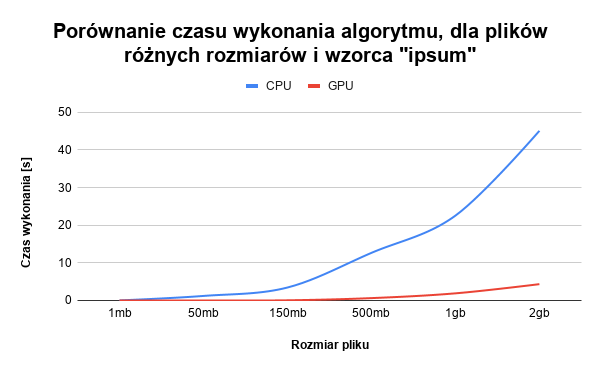
\includegraphics[width=\linewidth]{images/wykres41.png}
    \caption{Porównanie czasu wykonania obu wersji algorytmu, dla plików rożnych rozmiarów}
    \label{fig:chart_1}
\end{figure}

Na załączonym wykresie można zauważyć znaczną przewagę symultanicznej wersji algorytmu. Dla pliku o rozmiarze 2GB otrzymano aż 40 sekund zysku. Rysunek \ref{fig:chart_1} pokazuje również, że charekterystka zależności czasu wykonania od rozmiaru pliku dla algorytmu działającego na \textbf{GPU} rośnie wolniej od charakterystyki dla algorytmu działającego na \textbf{CPU}.

\subsection{Różna długość szukanego wzorca}

Pomiary dla wzorca o różnej długości dla pliku o rozmiarze 500MB zostały przeprowadzone w celu sprawdzenia, czy długość szukanej frazy nie ma drastycznego wpływu na czas wykonania algorytmu. Niestety, charakterystyka użytego algorytmu haszującego nie pozwoliła na wykonanie pomiarów dla wzorca posiadającego więcej niż 50 znaków, ze względu na przekroczenie maksymalnego zakresu zmiennej typu \textbf{long long int}. Uzyskane wyniki zostały przedstawione na rysunku \ref{fig:chart_2}.


\begin{figure}[H]
    \centering
    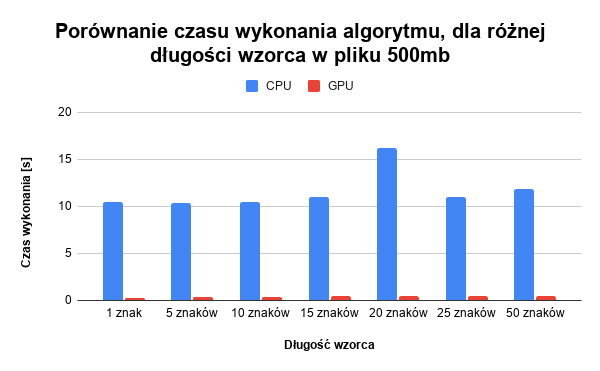
\includegraphics[width=\linewidth]{images/wykres42.png}
    \caption{Porównanie czasu wykonania obu wersji algorytmu, dla wzorca różnej długości}
    \label{fig:chart_2}
\end{figure}

Analizując wyniki przedstawione na rysunku \ref{fig:chart_2} można stwierdzić, że pomiary czasu wykonywania algorytmu dla wzorców o długości mniejszej niż 20 znaków oscylują wokół 10 sekund. Dla wzorca o długości 20 znaków obserwuje się najdłuższy czas wykonania algorytmu na \textbf{CPU}. Wynika to z wyboru specyficznego wzorca, którego hasz częściej zgadzał się z haszem porównywanych okien. W takim przypadku wartości funkcji haszującej były jednakowe, co skutkowało potrzebą wykonania dodatkowych operacji porównania. Dla pozostałych pomiarów obserwowalny jest nieznaczy wzrost czasu wykonywania wraz ze wzrostem długości wzorca.\\
Pomimo braku możliwości zbadania algorytmu dla dłuższych ciągów znaków, posiada on pewne cechy, które pozwalają antycypować jak będzie się zachowywał. W oparciu o wzór przedstawiony w podrozdziale \ref{subsec:parallelism} nie można dopuścić do przypadku, w którym \textit{$C_i$} \text{<} \textit{S}. Jedynym sposobem, który pozwala tego uniknąć, jest odpowiednie zmniejszenie liczby wątków, na których wykonywany jest algorytm. W najgorszym przypadku może to skutkować wykonywaniem całego programu w obrębie tylko jednego warp'a. Oznacza to, że potencjał karty graficznej byłby wykorzystany w małym procencie i prawdopodobnie uzyskanie gorszych rezultatów niż w przypadku \textbf{CPU}.

\subsection{Optymistyczne i pesymistyczne przypadki}

Dla algorytmu \textit{Rabina-Karpa} istnieją przypadki optymistyczne, których złożoność obliczeniowa wynosi \textit{O(m+n)} oraz pesymistyczne, których złożoność obliczeniowa wynosi \textit{$O(m*n)$}. Przypadek optymistyczny to taki, w którym hasz każdego porównywanego okna nie jest równy haszowi wzorca, co skutkuje brakiem operacji porównania tekstu, a więc również krótszym czasem wykonania. Natomiast pesymistyczne przypadki to takie, gdzie hasz każdego porównywanego okna jest równy haszowi wzorca co skutkuje, że porównywanie \say{znak po znaku} następuje za każdym razem. Taka sytuacja ma negatywny wpływ na wydajność. Przygotowane zestawy danych pozwoliły na zbadanie oraz porównanie czasu wykonania algorytmu dla takich przypadków, a uzyskane wyniki przedstawiono na rysunku \ref{fig:chart_3}.

\begin{figure}[H]
    \centering
    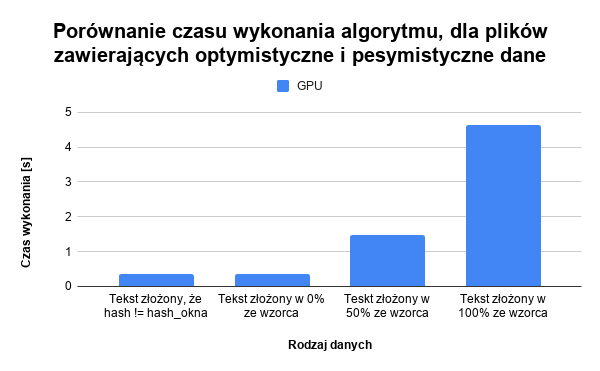
\includegraphics[width=\linewidth]{images/wykres43.png}
    \caption{Wyniki wersji na \textbf{GPU}, dla optymistycznych i pesymistycznych przypadków}
    \label{fig:chart_3}
\end{figure}

Na powyższym wykresie można zauważyć, że w przypadku pesymistycznym, algorytm działa wolniej aż 9-krotnie, niż dla przypadków optymistycznych. Widać również, że dla tekstu, w którym wystąpienie szukanego wzorca wynosiło \textit{$0\%$} otrzymano wyniki bardzo przybliżone do wyników dla danych optymistycznych. Spowodowane jet to niską częstotliwością występowania okien, których hasz zgadza się z haszem szukanego wzorca.